%\documentclass[
  bibliography=totoc,     % Literatur im Inhaltsverzeichnis
  captions=tableheading,  % Tabellenüberschriften
  titlepage=firstiscover, % Titelseite ist Deckblatt
]{scrartcl}

% Paket float verbessern
\usepackage{scrhack}

% Warnung, falls nochmal kompiliert werden muss
\usepackage[aux]{rerunfilecheck}

% unverzichtbare Mathe-Befehle
\usepackage{amsmath}
% viele Mathe-Symbole
\usepackage{amssymb}
% Erweiterungen für amsmath
\usepackage{mathtools}

% Fonteinstellungen
\usepackage{fontspec}
% Latin Modern Fonts werden automatisch geladen
% Alternativ zum Beispiel:
%\setromanfont{Libertinus Serif}
%\setsansfont{Libertinus Sans}
%\setmonofont{Libertinus Mono}

% Wenn man andere Schriftarten gesetzt hat,
% sollte man das Seiten-Layout neu berechnen lassen
\recalctypearea{}

% deutsche Spracheinstellungen
\usepackage[ngerman]{babel}


\usepackage[
  math-style=ISO,    % ┐
  bold-style=ISO,    % │
  sans-style=italic, % │ ISO-Standard folgen
  nabla=upright,     % │
  partial=upright,   % │
  mathrm=sym,        % ┘
  warnings-off={           % ┐
    mathtools-colon,       % │ unnötige Warnungen ausschalten
    mathtools-overbracket, % │
  },                       % ┘
]{unicode-math}

% traditionelle Fonts für Mathematik
\setmathfont{Latin Modern Math}
% Alternativ zum Beispiel:
%\setmathfont{Libertinus Math}

\setmathfont{XITS Math}[range={scr, bfscr}]
\setmathfont{XITS Math}[range={cal, bfcal}, StylisticSet=1]

% Zahlen und Einheiten
\usepackage[
  locale=DE,                   % deutsche Einstellungen
  separate-uncertainty=true,   % immer Unsicherheit mit \pm
  per-mode=symbol-or-fraction, % / in inline math, fraction in display math
]{siunitx}

% chemische Formeln
\usepackage[
  version=4,
  math-greek=default, % ┐ mit unicode-math zusammenarbeiten
  text-greek=default, % ┘
]{mhchem}

% richtige Anführungszeichen
\usepackage[autostyle]{csquotes}

% schöne Brüche im Text
\usepackage{xfrac}

% Standardplatzierung für Floats einstellen
\usepackage{float}
\floatplacement{figure}{htbp}
\floatplacement{table}{htbp}

% Floats innerhalb einer Section halten
\usepackage[
  section, % Floats innerhalb der Section halten
  below,   % unterhalb der Section aber auf der selben Seite ist ok
]{placeins}

% Seite drehen für breite Tabellen: landscape Umgebung
\usepackage{pdflscape}

% Captions schöner machen.
\usepackage[
  labelfont=bf,        % Tabelle x: Abbildung y: ist jetzt fett
  font=small,          % Schrift etwas kleiner als Dokument
  width=0.9\textwidth, % maximale Breite einer Caption schmaler
]{caption}
% subfigure, subtable, subref
\usepackage{subcaption}

% Grafiken können eingebunden werden
\usepackage{graphicx}

% schöne Tabellen
\usepackage{tabularray}
\UseTblrLibrary{booktabs, siunitx}

% Verbesserungen am Schriftbild
\usepackage{microtype}

% Literaturverzeichnis
\usepackage[
  backend=biber,
]{biblatex}
% Quellendatenbank
\addbibresource{lit.bib}
\addbibresource{programme.bib}

% Hyperlinks im Dokument
\usepackage[
  german,
  unicode,        % Unicode in PDF-Attributen erlauben
  pdfusetitle,    % Titel, Autoren und Datum als PDF-Attribute
  pdfcreator={},  % ┐ PDF-Attribute säubern
  pdfproducer={}, % ┘
]{hyperref}
% erweiterte Bookmarks im PDF
\usepackage{bookmark}

% Trennung von Wörtern mit Strichen
\usepackage[shortcuts]{extdash}

\author{%
  Vincent Wirsdörfer\\%
  \href{mailto:vincent.wirsdoerfer@udo.edu}{authorA@udo.edu}%
  \and%
  Joris Daus\\%
  \href{mailto:joris.daus@udo.edu}{authorB@udo.edu}%
}
\publishers{TU Dortmund – Fakultät Physik}


%\begin{document}
\section{Auswertung}
\label{sec:Auswertung}

%
%Mit Theorie vielleicht weg machen, wenn es in der Theorie schon vorgekommen ist.
%
%

Elementarer Bestandteil der Auswertung ist die Berechnung der effektiven Masse der Leitungselektronen in n-dotiertem 
Galliumarsenid. Zu Beginn wird jedoch die Analyse des Magnetfeldes in kleinen Abständen um die Probe aufgeführt.

%
%
%
%

\subsection{Magnetfeld an der Probe}
\noindent Für \autoref{eqn:Winkel_frei} wird das Magnetfeld an der Probe benötigt. Um dies zu bestimmen, 
werden die Daten aus \autoref{tab:magnetfeld} aufgetragen.

\begin{figure}[H]
    \centering
    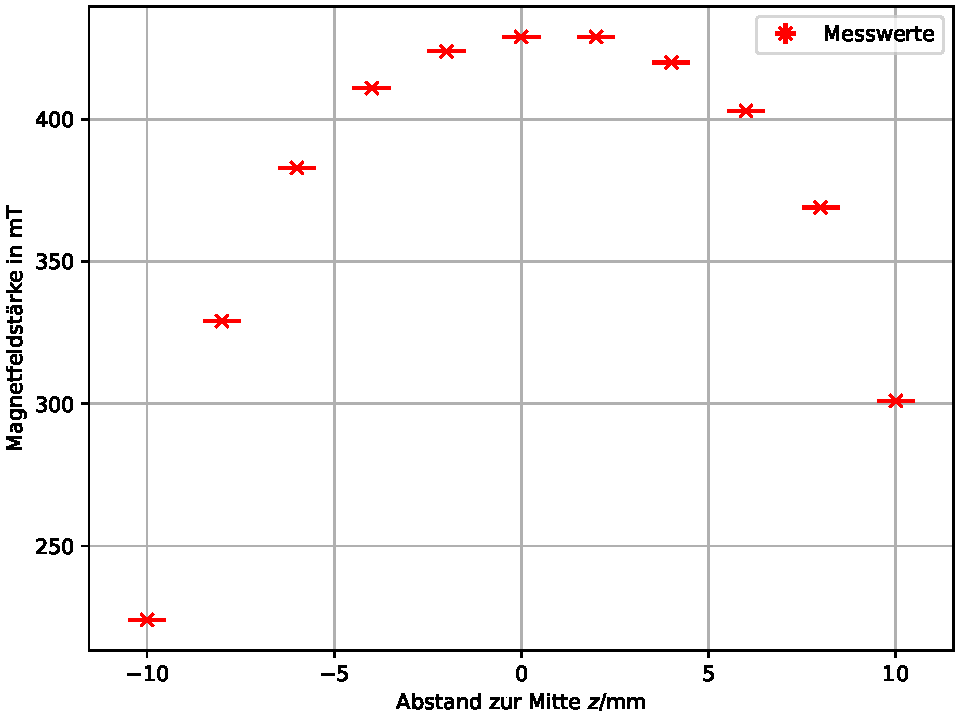
\includegraphics[width = 0.9\textwidth]{Magnetfeld.pdf}
    \caption{Magnetfeld im Inneren des Magneten in Abhängigkeit vom Abstand zur Mitte der Probe.}
    \label{fig:magnetfeld}
\end{figure}

\noindent Wie zu sehen ist, ist das Maximum des Magnetfelds genau am Ort der Probe. Das Magnetfeld 
direkt an der Probe beträgt somit 
%
%
% gleichen Wert wie in Rechnung nehmen
$B=\qty{429}{\milli \tesla}$.
%
%
%

\subsection{Winkelmessungen}
\noindent Im Folgenden werden nun die rohen Messdaten der Winkel gegen $\lambda^2$ aufgetragen, um diese 
zu sichten.

\begin{figure}[H]
    \centering
    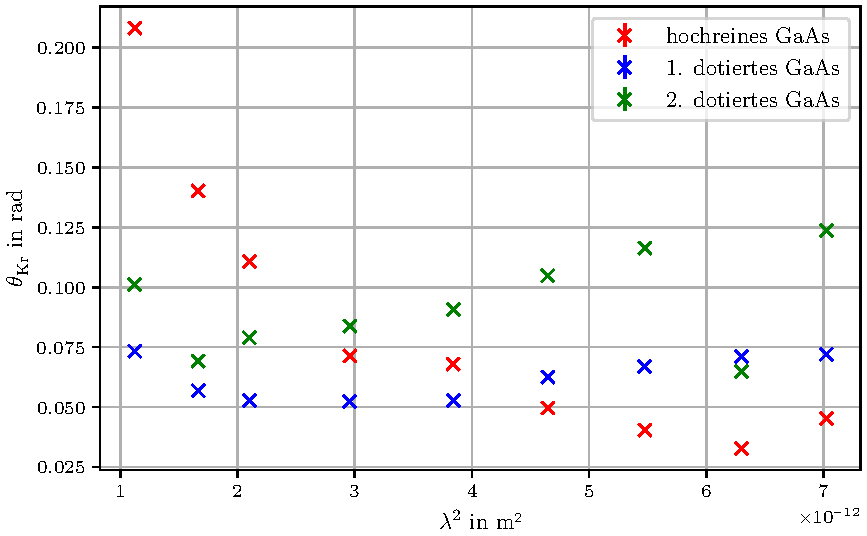
\includegraphics[width=0.9\textwidth]{Kristallwinkel.pdf}
    \caption{Messwerte aller Proben.}
    \label{fig:roh}
\end{figure}

\noindent Es ist zu sehen, dass es schon einige Ausreißer gibt. Dementsprechend wird später überprüft, welche 
Werte in die Rechnung genommen werden.\\
\noindent Da die absoluten Winkel des Goniometers nicht von Interesse sind, sondern nur der relative 
Winkel, um den die Polarisation gedreht wird, müssen diese noch bestimmt werden. Dieser lässt sich 
bestimmen, indem die Differenz der Winkel gebildet und halbiert wird.

\begin{equation}
    \centering
    \theta_\text{frei}=\frac{1}{2} \left(\theta_2 - \theta_1 \right)
    \label{eqn:theta_frei}
\end{equation}

\noindent Dies wird für alle drei Proben gebildet, da nur die relative Drehung wichtig ist. 
Die Drehung muss außerdem auf eine Drehung pro Strecke umgerechnet werden. Dies geschieht, indem der Drehwinkel 
durch die Dicke der Probe geteilt wird.
Um allen Einfluss, welcher nicht auf die Ladungsträgerdichte zurückzuführen ist, herauszurechnen, wird 
$\theta_\text{KR}$ des undotierten GaAs von $\theta_\text{KR}$ der dotierten GaAs Proben abgezogen. 
Dies geschieht für beide Proben und wird nun aufgetragen, um ausreißende Datenpunkte zu finden.

\begin{figure}[H]
    \centering
    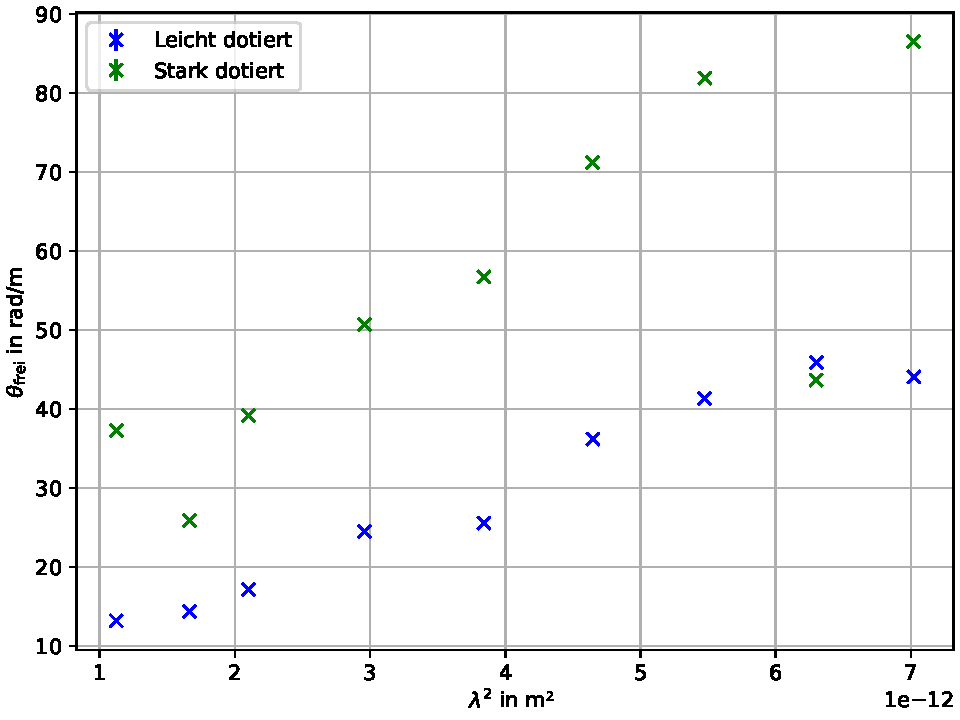
\includegraphics[width=0.9\textwidth]{Rohplot.pdf}
    \caption{Differenz der Winkel vor Ausfilterung.}
    \label{fig:pre}
\end{figure}

\noindent Hier ist zu sehen, dass der zweite und der achte Wert starke Abweichungen von den anderen Werten 
aufzeigen. Daher werden diese in den folgenden Berechnungen nicht mit gewertet. Es kann nun eine Ausgleichsrechnung 
durchgeführt werden, in der \autoref{eqn:Winkel_frei} gefittet wird. 

\begin{figure}[H]
    \centering
    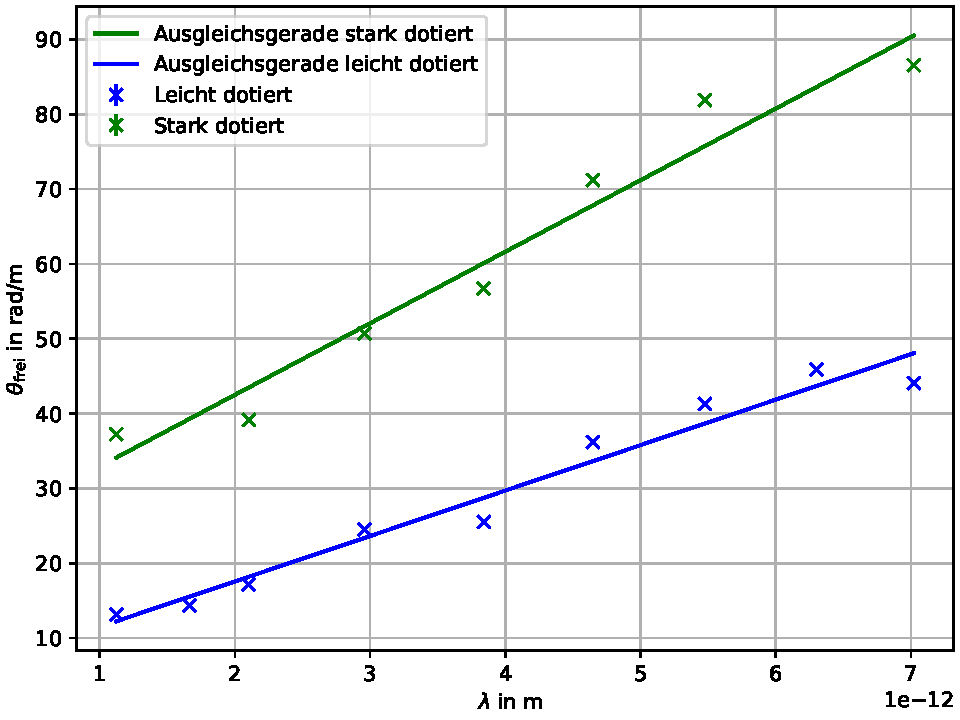
\includegraphics[width=0.9\textwidth]{LinRegress.pdf}
    \caption{Lineare Ausgleichsrechnung der freien Winkel.}
    \label{fig:LinRegress}
\end{figure}

\noindent Die Steigungen der stark und schwach dotierten  

\begin{align*}
    m_\text{stark}  &=\qty{9.6\pm0.9e12}{\radian \per \meter \squared}\\
    m_\text{schwach}&=\qty{6.1\pm0.4e12}{\radian \per \meter \squared}\\
\end{align*}

\noindent Wenn die Steigung nun mit dem Vorfaktor von \autoref{eqn:Winkel_frei} gleichgesetzt wird, ergibt sich

\begin{align*}
    m_\text{stark}  &=\frac{e_0^3}{8 \pi ^2 \varepsilon_0c^3} \frac{NB}{nm^*}\\
    m_\text{schwach}&=\frac{e_0^3}{8 \pi ^2 \varepsilon_0c^3} \frac{NB}{nm^*}\\
\end{align*}

\noindent Dies kann nun nach $m^*$ umgestellt werden. Es ergibt sich so für die effektive Masse:

\begin{align*}
    m_\text{stark}  &=\qty{9.00\pm0.40e-32}{\kilo \gram} = \num{0.0814\pm0.0030}m_e\\
    m_\text{schwach}&=\qty{7.42\pm0.27e-32}{\kilo \gram} = \num{0.0990\pm0.0050}m_e\\
\end{align*}




%\end{document}
